% Options for packages loaded elsewhere
\PassOptionsToPackage{unicode}{hyperref}
\PassOptionsToPackage{hyphens}{url}
%
\documentclass[
]{article}
\usepackage{lmodern}
\usepackage{amssymb,amsmath}
\usepackage{ifxetex,ifluatex}
\ifnum 0\ifxetex 1\fi\ifluatex 1\fi=0 % if pdftex
  \usepackage[T1]{fontenc}
  \usepackage[utf8]{inputenc}
  \usepackage{textcomp} % provide euro and other symbols
\else % if luatex or xetex
  \usepackage{unicode-math}
  \defaultfontfeatures{Scale=MatchLowercase}
  \defaultfontfeatures[\rmfamily]{Ligatures=TeX,Scale=1}
\fi
% Use upquote if available, for straight quotes in verbatim environments
\IfFileExists{upquote.sty}{\usepackage{upquote}}{}
\IfFileExists{microtype.sty}{% use microtype if available
  \usepackage[]{microtype}
  \UseMicrotypeSet[protrusion]{basicmath} % disable protrusion for tt fonts
}{}
\makeatletter
\@ifundefined{KOMAClassName}{% if non-KOMA class
  \IfFileExists{parskip.sty}{%
    \usepackage{parskip}
  }{% else
    \setlength{\parindent}{0pt}
    \setlength{\parskip}{6pt plus 2pt minus 1pt}}
}{% if KOMA class
  \KOMAoptions{parskip=half}}
\makeatother
\usepackage{xcolor}
\IfFileExists{xurl.sty}{\usepackage{xurl}}{} % add URL line breaks if available
\IfFileExists{bookmark.sty}{\usepackage{bookmark}}{\usepackage{hyperref}}
\hypersetup{
  pdftitle={Analysis},
  hidelinks,
  pdfcreator={LaTeX via pandoc}}
\urlstyle{same} % disable monospaced font for URLs
\usepackage[margin=1in]{geometry}
\usepackage{color}
\usepackage{fancyvrb}
\newcommand{\VerbBar}{|}
\newcommand{\VERB}{\Verb[commandchars=\\\{\}]}
\DefineVerbatimEnvironment{Highlighting}{Verbatim}{commandchars=\\\{\}}
% Add ',fontsize=\small' for more characters per line
\usepackage{framed}
\definecolor{shadecolor}{RGB}{248,248,248}
\newenvironment{Shaded}{\begin{snugshade}}{\end{snugshade}}
\newcommand{\AlertTok}[1]{\textcolor[rgb]{0.94,0.16,0.16}{#1}}
\newcommand{\AnnotationTok}[1]{\textcolor[rgb]{0.56,0.35,0.01}{\textbf{\textit{#1}}}}
\newcommand{\AttributeTok}[1]{\textcolor[rgb]{0.77,0.63,0.00}{#1}}
\newcommand{\BaseNTok}[1]{\textcolor[rgb]{0.00,0.00,0.81}{#1}}
\newcommand{\BuiltInTok}[1]{#1}
\newcommand{\CharTok}[1]{\textcolor[rgb]{0.31,0.60,0.02}{#1}}
\newcommand{\CommentTok}[1]{\textcolor[rgb]{0.56,0.35,0.01}{\textit{#1}}}
\newcommand{\CommentVarTok}[1]{\textcolor[rgb]{0.56,0.35,0.01}{\textbf{\textit{#1}}}}
\newcommand{\ConstantTok}[1]{\textcolor[rgb]{0.00,0.00,0.00}{#1}}
\newcommand{\ControlFlowTok}[1]{\textcolor[rgb]{0.13,0.29,0.53}{\textbf{#1}}}
\newcommand{\DataTypeTok}[1]{\textcolor[rgb]{0.13,0.29,0.53}{#1}}
\newcommand{\DecValTok}[1]{\textcolor[rgb]{0.00,0.00,0.81}{#1}}
\newcommand{\DocumentationTok}[1]{\textcolor[rgb]{0.56,0.35,0.01}{\textbf{\textit{#1}}}}
\newcommand{\ErrorTok}[1]{\textcolor[rgb]{0.64,0.00,0.00}{\textbf{#1}}}
\newcommand{\ExtensionTok}[1]{#1}
\newcommand{\FloatTok}[1]{\textcolor[rgb]{0.00,0.00,0.81}{#1}}
\newcommand{\FunctionTok}[1]{\textcolor[rgb]{0.00,0.00,0.00}{#1}}
\newcommand{\ImportTok}[1]{#1}
\newcommand{\InformationTok}[1]{\textcolor[rgb]{0.56,0.35,0.01}{\textbf{\textit{#1}}}}
\newcommand{\KeywordTok}[1]{\textcolor[rgb]{0.13,0.29,0.53}{\textbf{#1}}}
\newcommand{\NormalTok}[1]{#1}
\newcommand{\OperatorTok}[1]{\textcolor[rgb]{0.81,0.36,0.00}{\textbf{#1}}}
\newcommand{\OtherTok}[1]{\textcolor[rgb]{0.56,0.35,0.01}{#1}}
\newcommand{\PreprocessorTok}[1]{\textcolor[rgb]{0.56,0.35,0.01}{\textit{#1}}}
\newcommand{\RegionMarkerTok}[1]{#1}
\newcommand{\SpecialCharTok}[1]{\textcolor[rgb]{0.00,0.00,0.00}{#1}}
\newcommand{\SpecialStringTok}[1]{\textcolor[rgb]{0.31,0.60,0.02}{#1}}
\newcommand{\StringTok}[1]{\textcolor[rgb]{0.31,0.60,0.02}{#1}}
\newcommand{\VariableTok}[1]{\textcolor[rgb]{0.00,0.00,0.00}{#1}}
\newcommand{\VerbatimStringTok}[1]{\textcolor[rgb]{0.31,0.60,0.02}{#1}}
\newcommand{\WarningTok}[1]{\textcolor[rgb]{0.56,0.35,0.01}{\textbf{\textit{#1}}}}
\usepackage{graphicx,grffile}
\makeatletter
\def\maxwidth{\ifdim\Gin@nat@width>\linewidth\linewidth\else\Gin@nat@width\fi}
\def\maxheight{\ifdim\Gin@nat@height>\textheight\textheight\else\Gin@nat@height\fi}
\makeatother
% Scale images if necessary, so that they will not overflow the page
% margins by default, and it is still possible to overwrite the defaults
% using explicit options in \includegraphics[width, height, ...]{}
\setkeys{Gin}{width=\maxwidth,height=\maxheight,keepaspectratio}
% Set default figure placement to htbp
\makeatletter
\def\fps@figure{htbp}
\makeatother
\setlength{\emergencystretch}{3em} % prevent overfull lines
\providecommand{\tightlist}{%
  \setlength{\itemsep}{0pt}\setlength{\parskip}{0pt}}
\setcounter{secnumdepth}{-\maxdimen} % remove section numbering

\title{Analysis}
\author{}
\date{\vspace{-2.5em}}

\begin{document}
\maketitle

\hypertarget{variable-description}{%
\section{Variable Description}\label{variable-description}}

\begin{itemize}
\tightlist
\item
  \emph{author\_id}: user identifier
\item
  \emph{month}: period of reference
\item
  \emph{monthly\_commits}: total number of commits made in a month
\item
  \emph{monthly\_project}: number of different project a user commited
  in a month
\item
  \emph{first\_commit}: month in which user made the first recorded
  commit
\item
  \emph{last\_commit}: month in which user made the last recorded commit
\item
  \emph{total\_commits}: total number of commits made by a user over
  time
\item
  \emph{number\_project}: total number of projects an user made
  contribution to
\item
  \emph{time active}: number of days between first and last commit
\end{itemize}

\hypertarget{multitasking}{%
\section{Multitasking}\label{multitasking}}

\begin{Shaded}
\begin{Highlighting}[]
\NormalTok{loc <-}\StringTok{ 'C:/Users/mmore/Dropbox/Econometrics II - TA/Project/GitHub/Data/commits/productive_users_50_2.csv'}
\NormalTok{df_pu <-}\StringTok{ }\KeywordTok{read.csv}\NormalTok{(loc)}
\end{Highlighting}
\end{Shaded}

\begin{Shaded}
\begin{Highlighting}[]
\KeywordTok{hist}\NormalTok{(df_pu}\OperatorTok{$}\NormalTok{monthly_project[df_pu}\OperatorTok{$}\NormalTok{monthly_project }\OperatorTok{>}\StringTok{ }\DecValTok{0} \OperatorTok{&}\StringTok{ }\NormalTok{df_pu}\OperatorTok{$}\NormalTok{monthly_project }\OperatorTok{<=}\StringTok{ }\DecValTok{20}\NormalTok{],}
     \DataTypeTok{xlab=}\StringTok{'N. monthly projects'}\NormalTok{,}
     \DataTypeTok{ylab=}\StringTok{'Frequency'}\NormalTok{,}
     \DataTypeTok{main=}\StringTok{'Distribution of N. monthly projects, Per User'}\NormalTok{)}
\end{Highlighting}
\end{Shaded}

\includegraphics{analysis_productive_users_files/figure-latex/unnamed-chunk-3-1.pdf}

\begin{Shaded}
\begin{Highlighting}[]
\NormalTok{multi_task_t <-}\StringTok{ }\DecValTok{2}

\NormalTok{tot_active <-}\StringTok{ }\NormalTok{df_pu }\OperatorTok\StringTok{ }\KeywordTok{filter}\NormalTok{(monthly_project}\OperatorTok{>=}\DecValTok{1}\NormalTok{) }\OperatorTok
\StringTok{                        }\KeywordTok{summarise}\NormalTok{(}\KeywordTok{n}\NormalTok{())}
\NormalTok{tot_active_multi <-}\StringTok{ }\NormalTok{df_pu }\OperatorTok\StringTok{ }\KeywordTok{filter}\NormalTok{(monthly_project}\OperatorTok{>=}\NormalTok{multi_task_t) }\OperatorTok
\StringTok{                        }\KeywordTok{summarise}\NormalTok{(}\KeywordTok{n}\NormalTok{())  }
  
\NormalTok{N_obs <-}\StringTok{ }\KeywordTok{nrow}\NormalTok{(df_pu)}
\NormalTok{period_active <-}\StringTok{ }\KeywordTok{round}\NormalTok{(}\KeywordTok{as.numeric}\NormalTok{(tot_active}\OperatorTok{/}\KeywordTok{nrow}\NormalTok{(df_pu))}\OperatorTok{*}\DecValTok{100}\NormalTok{,}\DecValTok{2}\NormalTok{)}
\NormalTok{period_multi_task <-}\StringTok{ }\KeywordTok{round}\NormalTok{(}\KeywordTok{as.numeric}\NormalTok{(tot_active_multi}\OperatorTok{/}\NormalTok{tot_active)}\OperatorTok{*}\DecValTok{100}\NormalTok{,}\DecValTok{2}\NormalTok{)    }
\end{Highlighting}
\end{Shaded}

We define an user \emph{i} as active in month \emph{t} if the user has
contributed to at least one project \emph{j}. We define that agent
\emph{i} did multi-tasking in month \emph{t} if she contributed to at
least two different projects. In the selected sample, we have:

\begin{itemize}
\tightlist
\item
  3116540 pair of user-month observations
\item
  18.06\% of the pairs \emph{(i,t)} (user-month) have at least one
  commit, i.e.~the user \emph{i} is active is active in month \emph{t}
\item
  26.13\% of the pairs \emph{(i,t)} (user-month) in which usere is
  active are subject to multitasking.\\
\item
  In total, we have 4.72\% observations in which agents perform
  multi-tasking
\end{itemize}

\begin{Shaded}
\begin{Highlighting}[]
\NormalTok{multi_task_t <-}\StringTok{ }\DecValTok{2}
\NormalTok{threshold <-}\StringTok{ }\DecValTok{500}

\NormalTok{tot_active_}\DecValTok{500}\NormalTok{ <-}\StringTok{ }\NormalTok{df_pu }\OperatorTok\StringTok{ }\KeywordTok{filter}\NormalTok{(monthly_project}\OperatorTok{>=}\DecValTok{1}\NormalTok{) }\OperatorTok
\StringTok{                            }\KeywordTok{filter}\NormalTok{(total_commits}\OperatorTok{>=}\NormalTok{threshold) }\OperatorTok
\StringTok{                            }\KeywordTok{summarise}\NormalTok{(}\KeywordTok{n}\NormalTok{())}

\NormalTok{tot_active_multi_}\DecValTok{500}\NormalTok{ <-}\StringTok{ }\NormalTok{df_pu }\OperatorTok\StringTok{ }
\StringTok{                    }\KeywordTok{filter}\NormalTok{(total_commits}\OperatorTok{>=}\NormalTok{threshold) }\OperatorTok
\StringTok{                    }\KeywordTok{filter}\NormalTok{(monthly_project}\OperatorTok{>=}\NormalTok{multi_task_t) }\OperatorTok
\StringTok{                    }\KeywordTok{summarise}\NormalTok{(}\KeywordTok{n}\NormalTok{())  }

\NormalTok{N_obs_}\DecValTok{500}\NormalTok{ <-}\StringTok{ }\NormalTok{df_pu }\OperatorTok
\StringTok{             }\KeywordTok{filter}\NormalTok{(total_commits}\OperatorTok{>=}\NormalTok{threshold)}\OperatorTok
\StringTok{             }\KeywordTok{summarise}\NormalTok{(}\KeywordTok{n}\NormalTok{())}

\NormalTok{N_obs_}\DecValTok{500}\NormalTok{ <-}\StringTok{ }\KeywordTok{as.numeric}\NormalTok{(N_obs_}\DecValTok{500}\NormalTok{)}


\NormalTok{period_active_}\DecValTok{500}\NormalTok{ <-}\StringTok{ }\KeywordTok{round}\NormalTok{(}\KeywordTok{as.numeric}\NormalTok{(tot_active_}\DecValTok{500}\OperatorTok{/}\NormalTok{N_obs_}\DecValTok{500}\NormalTok{)}\OperatorTok{*}\DecValTok{100}\NormalTok{,}\DecValTok{2}\NormalTok{)}
\NormalTok{period_multi_task_}\DecValTok{500}\NormalTok{ <-}\StringTok{ }\KeywordTok{round}\NormalTok{(}\KeywordTok{as.numeric}\NormalTok{(tot_active_multi_}\DecValTok{500}\OperatorTok{/}\NormalTok{tot_active_}\DecValTok{500}\NormalTok{)}\OperatorTok{*}\DecValTok{100}\NormalTok{,}\DecValTok{2}\NormalTok{)    }
\end{Highlighting}
\end{Shaded}

In we restrict to users who have made at least 500 commits in their
history, we have:

\begin{itemize}
\item
\item
  425897 pair of user-month observations
\item
  38.47\% of the pairs \emph{(i,t)} (user-month) have at least one
  commit, i.e.~the user \emph{i} is active is active in month \emph{t}
\item
  38.72\% of the pairs \emph{(i,t)} (user-month) in which usere is
  active are subject to multitasking.\\
\item
  In total, we have 14.9\% observations in which agents perform
  multi-tasking
\end{itemize}

\begin{Shaded}
\begin{Highlighting}[]
\NormalTok{thresholds <-}\StringTok{ }\KeywordTok{seq}\NormalTok{(}\DecValTok{100}\NormalTok{,}\DecValTok{1500}\NormalTok{,}\DecValTok{100}\NormalTok{)}
\NormalTok{store <-}\StringTok{ }\KeywordTok{matrix}\NormalTok{(}\DecValTok{0}\NormalTok{,}\DecValTok{5}\NormalTok{,}\KeywordTok{length}\NormalTok{(thresholds))}

\NormalTok{i <-}\StringTok{ }\DecValTok{1}

\ControlFlowTok{for}\NormalTok{ (threshold }\ControlFlowTok{in}\NormalTok{ thresholds)\{}
  
\NormalTok{  store[}\DecValTok{1}\NormalTok{,i] <-}\StringTok{ }\KeywordTok{as.numeric}\NormalTok{(df_pu }\OperatorTok\StringTok{ }\KeywordTok{filter}\NormalTok{(total_commits}\OperatorTok{>=}\NormalTok{threshold) }\OperatorTok\StringTok{ }\KeywordTok{summarise}\NormalTok{(}\KeywordTok{n_distinct}\NormalTok{(author_id)))}
\NormalTok{  df_temp <-}\StringTok{ }\NormalTok{df_pu }\OperatorTok\StringTok{ }\KeywordTok{filter}\NormalTok{(total_commits}\OperatorTok{>=}\NormalTok{threshold) }\OperatorTok\StringTok{ }
\StringTok{                                     }\KeywordTok{group_by}\NormalTok{(author_id) }\OperatorTok\StringTok{ }
\StringTok{                                     }\KeywordTok{mutate}\NormalTok{(}\DataTypeTok{multi =} \KeywordTok{max}\NormalTok{(monthly_project)) }\OperatorTok
\StringTok{                                     }\KeywordTok{filter}\NormalTok{(multi}\OperatorTok{>}\DecValTok{1}\NormalTok{) }
  
\NormalTok{  store[}\DecValTok{2}\NormalTok{,i] <-}\StringTok{ }\KeywordTok{round}\NormalTok{(}\KeywordTok{length}\NormalTok{(}\KeywordTok{unique}\NormalTok{(df_temp}\OperatorTok{$}\NormalTok{author_id))}\OperatorTok{/}\NormalTok{store[}\DecValTok{1}\NormalTok{,i] }\OperatorTok{*}\StringTok{ }\DecValTok{100}\NormalTok{,}\DecValTok{2}\NormalTok{)}
  
\NormalTok{  df_temp <-}\StringTok{ }\NormalTok{df_pu }\OperatorTok\StringTok{ }\KeywordTok{filter}\NormalTok{(total_commits}\OperatorTok{>=}\NormalTok{threshold) }
\NormalTok{  store[}\DecValTok{3}\NormalTok{,i] <-}\StringTok{ }\KeywordTok{nrow}\NormalTok{(df_temp)}
  
\NormalTok{  df_temp <-}\StringTok{ }\NormalTok{df_pu }\OperatorTok\StringTok{ }\KeywordTok{filter}\NormalTok{(monthly_project}\OperatorTok{>}\DecValTok{1}\NormalTok{) }\OperatorTok
\StringTok{                       }\KeywordTok{filter}\NormalTok{(total_commits}\OperatorTok{>=}\NormalTok{threshold) }
  
\NormalTok{  store[}\DecValTok{4}\NormalTok{,i] <-}\StringTok{ }\KeywordTok{round}\NormalTok{(}\KeywordTok{nrow}\NormalTok{(df_temp)  }\OperatorTok{*}\StringTok{ }\DecValTok{100} \OperatorTok{/}\StringTok{ }\NormalTok{store[}\DecValTok{3}\NormalTok{,i],}\DecValTok{2}\NormalTok{) }
\NormalTok{  df_temp <-}\StringTok{ }\NormalTok{df_pu }\OperatorTok\StringTok{ }\KeywordTok{filter}\NormalTok{(monthly_project}\OperatorTok{>=}\DecValTok{1}\NormalTok{) }\OperatorTok
\StringTok{                       }\KeywordTok{filter}\NormalTok{(total_commits}\OperatorTok{>=}\NormalTok{threshold) }
  
\NormalTok{  store[}\DecValTok{5}\NormalTok{,i] <-}\StringTok{ }\KeywordTok{round}\NormalTok{(}\KeywordTok{nrow}\NormalTok{(df_temp) }\OperatorTok{*}\StringTok{ }\DecValTok{100} \OperatorTok{/}\StringTok{ }\NormalTok{store[}\DecValTok{3}\NormalTok{,i],}\DecValTok{2}\NormalTok{)}

\NormalTok{  i <-}\StringTok{ }\NormalTok{i }\OperatorTok{+}\StringTok{ }\DecValTok{1}

\NormalTok{\}}

\KeywordTok{rownames}\NormalTok{(store) <-}\StringTok{ }\KeywordTok{c}\NormalTok{(}\StringTok{'N.Users'}\NormalTok{,}\StringTok{'Share of Users Multitasking at least 1 month'}\NormalTok{,}\StringTok{'N. Obs'}\NormalTok{,}\StringTok{'Share of Obs. with multi-tasking'}\NormalTok{,}\StringTok{'Share of Obs. with Commits'}\NormalTok{)}
\KeywordTok{colnames}\NormalTok{(store) <-}\StringTok{ }\KeywordTok{paste}\NormalTok{(}\StringTok{'>='}\NormalTok{,thresholds,}\DataTypeTok{sep=}\StringTok{''}\NormalTok{)}
\KeywordTok{View}\NormalTok{(store)}
\end{Highlighting}
\end{Shaded}

\begin{Shaded}
\begin{Highlighting}[]
\KeywordTok{plot}\NormalTok{(thresholds,store[}\DecValTok{1}\NormalTok{,],}
     \DataTypeTok{xlab=}\StringTok{'Lower Bound on Total N. of Commits'}\NormalTok{,}
     \DataTypeTok{ylab=}\StringTok{''}\NormalTok{,}
     \DataTypeTok{main=}\KeywordTok{rownames}\NormalTok{(store)[}\DecValTok{1}\NormalTok{])}
\end{Highlighting}
\end{Shaded}

\includegraphics{analysis_productive_users_files/figure-latex/unnamed-chunk-6-1.pdf}

\begin{Shaded}
\begin{Highlighting}[]
\KeywordTok{plot}\NormalTok{(thresholds,store[}\DecValTok{3}\NormalTok{,],}
     \DataTypeTok{xlab=}\StringTok{'Lower Bound on Total N. of Commits'}\NormalTok{,}
     \DataTypeTok{ylab=}\StringTok{''}\NormalTok{,}
     \DataTypeTok{main=}\KeywordTok{rownames}\NormalTok{(store)[}\DecValTok{3}\NormalTok{])}
\end{Highlighting}
\end{Shaded}

\includegraphics{analysis_productive_users_files/figure-latex/unnamed-chunk-6-2.pdf}

\begin{Shaded}
\begin{Highlighting}[]
\KeywordTok{plot}\NormalTok{(thresholds,store[}\DecValTok{2}\NormalTok{,],}
     \DataTypeTok{xlab=}\StringTok{'Lower Bound on Total N. of Commits'}\NormalTok{,}
     \DataTypeTok{ylab=}\StringTok{''}\NormalTok{,}
     \DataTypeTok{main=}\KeywordTok{rownames}\NormalTok{(store)[}\DecValTok{2}\NormalTok{])}
\end{Highlighting}
\end{Shaded}

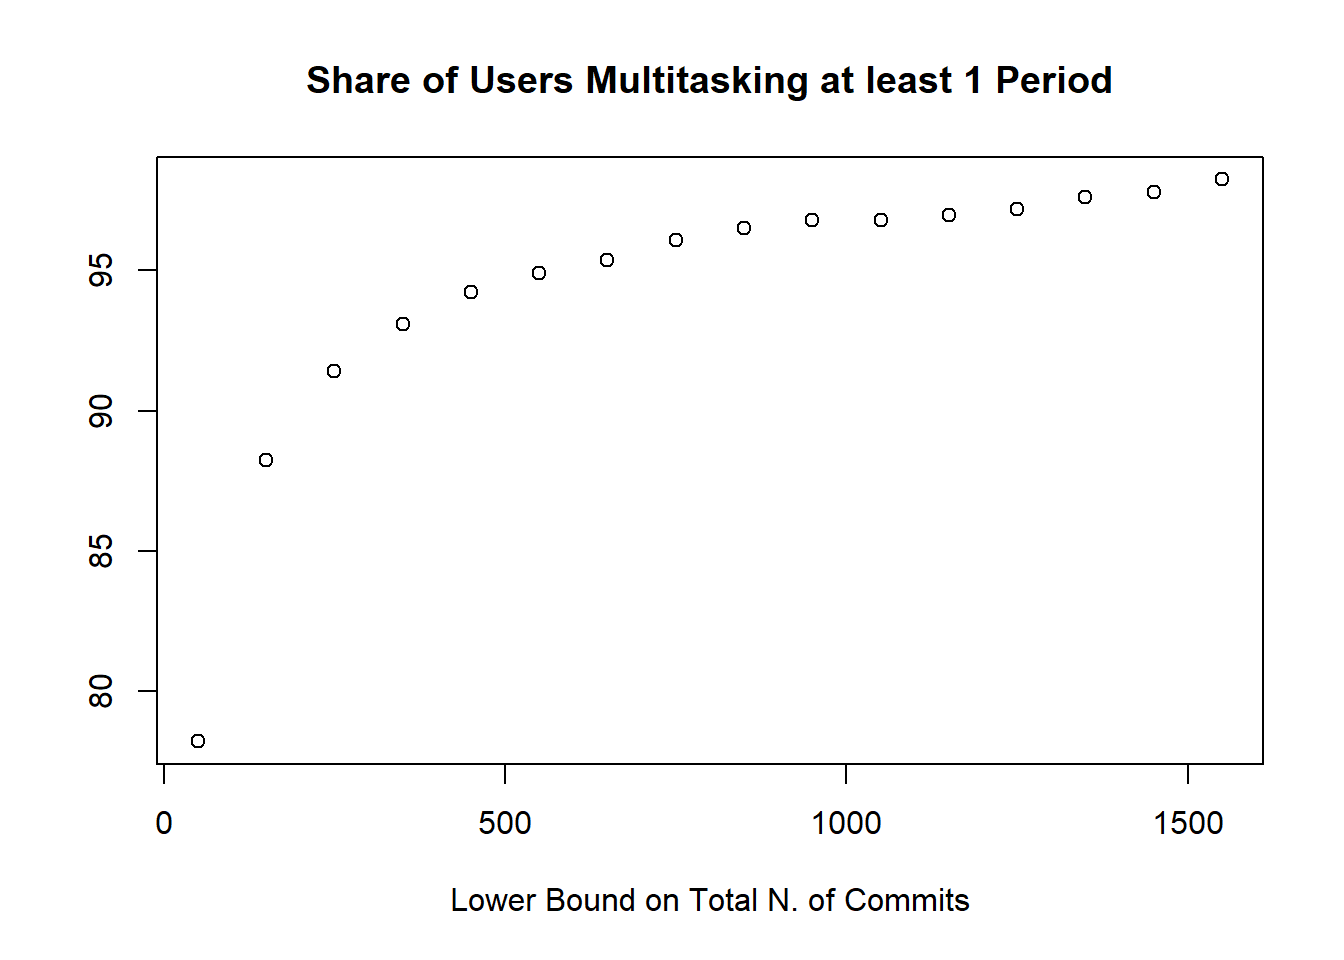
\includegraphics{analysis_productive_users_files/figure-latex/unnamed-chunk-6-3.pdf}

\begin{Shaded}
\begin{Highlighting}[]
\KeywordTok{plot}\NormalTok{(thresholds,store[}\DecValTok{5}\NormalTok{,],}
     \DataTypeTok{xlab=}\StringTok{'Lower Bound on Total N. of Commits'}\NormalTok{,}
     \DataTypeTok{ylab=}\StringTok{'%'}\NormalTok{,}
     \DataTypeTok{main=}\KeywordTok{rownames}\NormalTok{(store)[}\DecValTok{5}\NormalTok{])}
\end{Highlighting}
\end{Shaded}

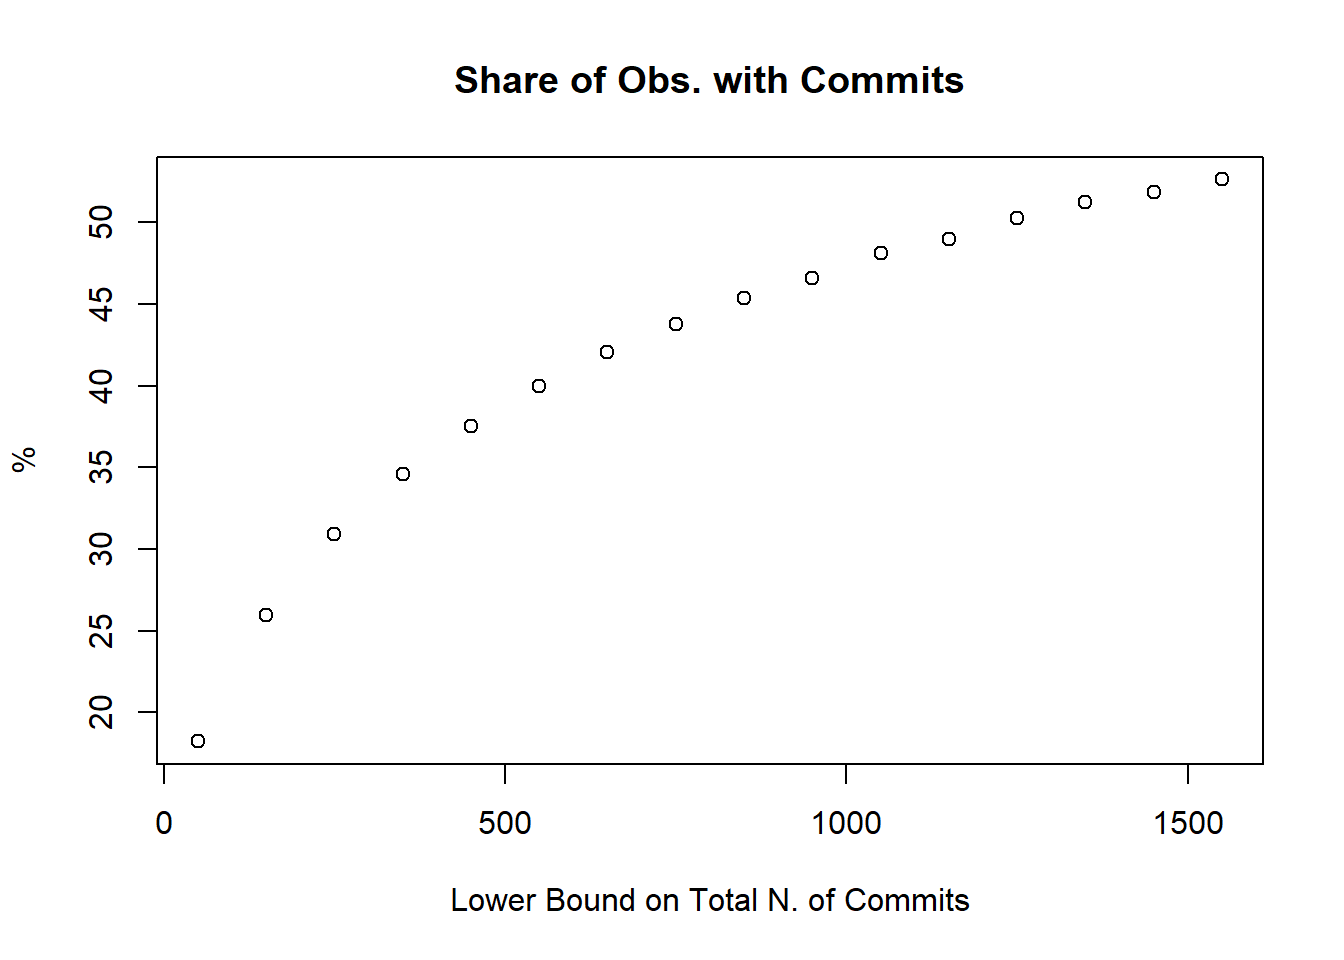
\includegraphics{analysis_productive_users_files/figure-latex/unnamed-chunk-6-4.pdf}

\begin{Shaded}
\begin{Highlighting}[]
\KeywordTok{plot}\NormalTok{(thresholds,store[}\DecValTok{4}\NormalTok{,],}
     \DataTypeTok{xlab=}\StringTok{'Lower Bound on Total N. of Commits'}\NormalTok{,}
     \DataTypeTok{ylab=}\StringTok{'%'}\NormalTok{,}
     \DataTypeTok{main=}\KeywordTok{rownames}\NormalTok{(store)[}\DecValTok{4}\NormalTok{])}
\end{Highlighting}
\end{Shaded}

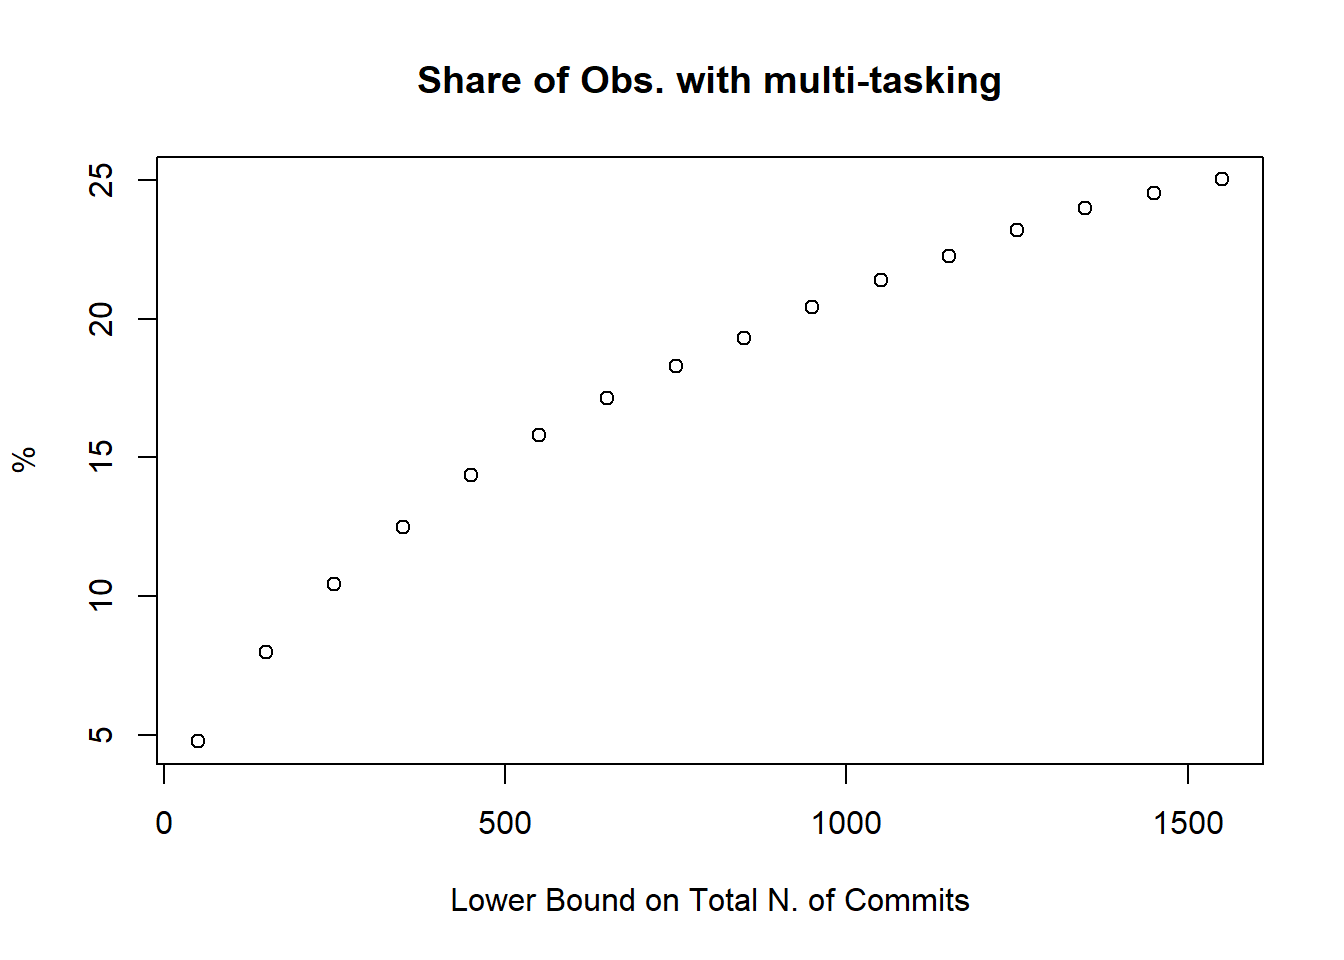
\includegraphics{analysis_productive_users_files/figure-latex/unnamed-chunk-6-5.pdf}

\end{document}
